% !TeX spellcheck = de_AT_frami
\section{Nichtlineare Gleichungssysteme}
	\begin{enumerate}
		\item \textbf{Beschreiben Sie das Newton-Verfahren in einer Veränderlichen. Skizze!} \\
			Es sei \(f:(a,b)\rightarrow\mathbb{R}\) eine stetig differenzierbare Funktion und \(x^\star\) eine einfache Nullstelle von f, d.h.
			\begin{align*}
				f(x^\star)=0 \quad \text{und} \quad f'(x^\star)\neq 0.
			\end{align*}
			Weiters sei \(x_0\) eine (grobe) Näherung an die gesuchte Nullstelle \(x^\star\) und \(f'(x_0)\neq 0\).
			Man bestimmt die Tangente im Punkt \((x_0,f(x_0))\) an den Graphen der Funktion \(f\) und berechnet deren Nullstelle \(x_1\). Die Nullstelle \(x_1\) der Tangente ist eine neue und hoffentlich bessere Näherung an die Nullstelle \(x^\star\) von \(f\).
			\begin{figure}[htbp]
				\centering
				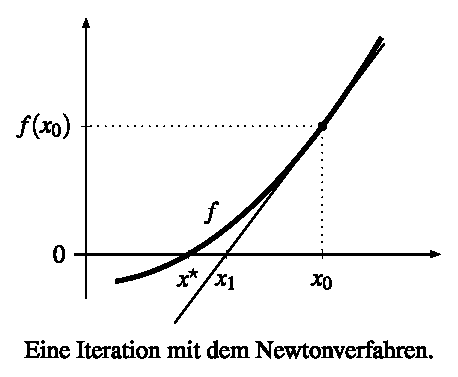
\includegraphics[width=0.35\linewidth]{Kap6_1}
			\end{figure}\\
			Nun gilt 
			\begin{align*}
				\frac{f(x_0)-0}{x_0-x_1}=f'(x_0) \Rightarrow x_1=x_0-\frac{f(x_0)}{f'(x_0)}
			\end{align*}
			Allgemein Formuliert:
			\begin{align*}
				x_0 &= \text{Startwert mit } f'(x_0)\neq 0 \\
				x_{k+1} &= x_k-\frac{f(x_k)}{f'(x_k)}, k\geq0
			\end{align*}
		\item \textbf{Wie ist das Newton-Verfahren in mehreren Veränderlichen definiert?}
			\begin{align*}
				x^{(0)} &= \text{Startwert mit } f'(x^{(0)}) \text{ invertierbar.} \\
				\text{löse } f'(x^{(k)})\cdot \Delta^{(k)} &= -f(x^{(k)}), \quad \text{mit } \Delta x^{(0)}=x^{(1)}-x^{(0)} \\
				x^{(k+1)} &= x^{(k)} +  \Delta x^{(k)}, \quad k\geq 0
			\end{align*}
			Falls \(\norm{\Delta x^{(k)}}\leq\text{TOL} \) wird das Verfahren abgebrochen und \(x^{(k+1)}\) als numerisches Ergebnis Akzeptiert.
		
		\item \textbf{Wie schnell konvergiert das Newton-Verfahren? Welche Voraussetzungen muss der Startwert erfüllen?} \\
			Die Funktion \(f\) sei in einer Umgebung von \(x^\star\) zweimal stetig differenzierbar und es gelte \(f(x^\star) =0\) und \(\det f'(x^\star)\neq 0\). Dann gilt
			\begin{align*}
				\norm{x^{(k+1)}-x^\star}\leq C\cdot \norm{x^{(k)}-x^\star}^2.
			\end{align*}
		
		\item \textbf{Wie ist das Gauß-Newton-Verfahren definiert?}
			\begin{align*}
			x^{(0)} &= \text{Startwert} \\
			\text{löse } f'(x^{(k)})^\text{T}f'(x^{(k)}) \cdot \Delta^{(k)} &= -f(x^{(k)})^\text{T}f(x^{(k)}), \quad \text{mit } \Delta x^{(0)}=x^{(1)}-x^{(0)} \\
			x^{(k+1)} &= x^{(k)} +  \Delta x^{(k)}, \quad k\geq 0
			\end{align*}
			Falls \(\norm{\Delta x^{(k)}}\leq\text{TOL} \) wird das Verfahren abgebrochen und \(x^{(k+1)}\) als numerisches Ergebnis Akzeptiert.
		
		\item \textbf{Wie ist das Konvergenzverhalten des Gauß-Newton-Verfahrens?} \\
			Es gibt Konstanten \(C_1>0\) und \(C_2>0\), sodass in der Nähe von \(x^\star\) gilt:
			\begin{align*}
				\norm{x^{(k+1)}-x^\star}\leq C_1\cdot f(x^\star)\cdot \norm{x^{(k)}-x^\star} + C_2\cdot \norm{x^{(k)}-x^\star}^2.
			\end{align*}
			Was liest man daraus?
			\begin{enumerate}
				\item[(1)] Die Konvergenz ist im Allgemeinen nur linear wegen \(C_1\cdot f(x^\star)\cdot \norm{x^{(k)}-x^\star}\).
				\item[(2)] Falls \(f(x^\star)=0\) (Die Gleichungen sind in diesem Fall kompatibel, d.h. nicht widersprüchlich), dann ist die Konvergenz sogar quadratisch, weil \(C_1\cdot f(x^\star)\cdot \norm{x^{(k)}-x^\star}\) wegfällt.
				\item[(3)] Falls \(f(x^\star)\) zu groß ist, dann divergiert das Verfahren.
			\end{enumerate}
		
	\end{enumerate}